%%%%%%%%%---Packages and document settings---%%%%%%%%%
\documentclass[twoside,twocolumn]{article}

  \usepackage{blindtext}      % Package to generate dummy text throughout this template 
  
  \usepackage[sc]{mathpazo}   % Use the Palatino font
  \linespread{1.05}           % Line spacing - Palatino needs more space between lines
  \usepackage[T1]{fontenc}    % Use 8-bit encoding that has 256 glyphs
  \usepackage{microtype}      % Slightly tweak font spacing for aesthetics
  
  \usepackage[spanish,es-tabla]{babel} % Language hyphenation and typographical rules
  \usepackage[utf8]{inputenc} % para poder utilizar acentos sin que te jodan
  
  \usepackage[hmarginratio=1:1,top=32mm,columnsep=20pt]{geometry}     % Document margins
  \usepackage[hang, small,labelfont=bf,up,textfont=it,up]{caption}    % Custom captions under/above floats in tables or figures
  \usepackage{booktabs}       % Horizontal rules in tables
  
  \usepackage{lettrine}       % The lettrine is the first enlarged letter at the beginning of the text
  
  \usepackage{enumitem}       % Customized lists
  \setlist[itemize]{noitemsep}  % Make itemize lists more compact
  
  \usepackage{mathtools}
  \DeclarePairedDelimiter\bra{\langle}{\rvert}        % Para notación de Dirac
  \DeclarePairedDelimiter\ket{\lvert}{\rangle}
  \DeclarePairedDelimiterX\braket[2]{\langle}{\rangle}{#1 \delimsize\vert #2}

  \usepackage{abstract}       % Allows abstract customization
  \renewcommand{\abstractnamefont}{\normalfont\bfseries}      % Set the "Abstract" text to bold
  \renewcommand{\abstracttextfont}{\normalfont\small\itshape} % Set the abstract itself to small italic text
  
  \usepackage{titlesec}                                   % Allows customization of titles
  \renewcommand\thesection{\Roman{section}}               % Roman numerals for the sections
  \renewcommand\thesubsection{\roman{subsection}}         % roman numerals for subsections
  \renewcommand\thesubsubsection{\arabic{subsubsection}}   % roman numerals for subsections
  \titleformat{\section}[block]{\Large\scshape\centering}{\thesection.}{1em}{}    % Change the look of the section titles
  \titleformat{\subsection}[block]{\large}{\thesubsection.}{1em}{}                % Change the look of the section titles
  \titleformat{\subsubsection}[block]{\it}{\quad\footnotesize\thesubsubsection.}{0.5em}{}                % Change the look of the section titles
  %\titleformat{\paragraph}[block]{\it}{\quad\footnotesize:}{0.1em}{}                % Change the look of the section titles

  \usepackage{fancyhdr}     % Headers and footers
  \pagestyle{fancy}         % All pages have headers and footers
  \fancyhead{}              % Blank out the default header
  %\fancyfoot{}              % Blank out the default footer
  \fancyhead[C]{Detección de partículas con CMOS $\bullet$ Mayo 2018 $\bullet$ D. F. Balmaceda}   % Custom header text
  %\fancyfoot[RO,LE]{\thepage} % Custom footer text
  
  \usepackage{titling}      % Customizing the title section
  
  \usepackage{hyperref}     % For hyperlinks in the PDF
  \usepackage{graphics}     % standard graphics specifications
  \usepackage{graphicx}     % alternative graphics specifications
  \usepackage{longtable}    % helps with long table options
  \usepackage{svg}          % para gráficos .svg
  \usepackage[binary-units=true]{siunitx}      % para las unidades
  \usepackage{datetime}


%%%%%%%%%---Title, authors, date & abstract---%%%%%%%%%
\title{Análisis de interacciones de partículas mediante implementación de una librería para su detección con sensores CMOS}
  \author{%
    \textsc{Darío Federico Balmaceda} \\[1ex]     %  Your name
    \normalsize Laboratorio Detección de Partículas y Radiación. Centro Atómico Bariloche \\        %  Your institution
    \normalsize \href{mailto:leschatten@gmail.com}{\texttt{leschatten@gmail.com}}                   %  Your email address
  }
  \date{\today}
  \renewcommand{\maketitlehookd}{
    \begin{abstract}
      Se utilizaron sensores CMOS para la detección de eventos con partículas para una descripción cualitativa y esquemática.
        Se analizó la dependencia con los distintos parámetros de la cámara y en base a esto se decidió una configuración de trabajo.

      Gracias a esto se pudo caracterizar y calibrar el sensor para la configuración utilizada mediante la implementación de la librería
        en C++ con filosofía de Programación Orientada a Objetos.
        Utilizando esta librería se observó la presencia de eventos producidos por rayos cósmicos y
        se observaron los picos $K_{\alpha}$ y $K_{\beta}$ del Cu y los picos $K_{\alpha}$ del Fe y Ca.
      %TODO: ABSTRACT
    \end{abstract}
  }

  \setlength{\droptitle}{-4\baselineskip}                 % Move the title up
  \pretitle{\begin{center}\Large\bfseries}                 % Article title formatting
  \posttitle{\end{center}}                                % Article title closing formatting

%
  %%%%%%%%%%%%%%%%%%%%%%%%%%%%%%%%%%%%%%%%%%
  %%%%                                 %%%%%
  %%%%  And now, begin the document... %%%%%
  %%%%                                 %%%%%
  %%%%%%%%%%%%%%%%%%%%%%%%%%%%%%%%%%%%%%%%%%
\begin{document}
  
  \maketitle              % Print the title
  
  %%%%%%%%%%%%%%%%%%%%%%%%%%%%%%%%%%%%%%%%%%%%%%%%%%%
  \section{Introducción}\label{sec:intro}
    \lettrine[nindent=0em,lines=3]{L}os sensores de imágenes CMOS son ampliamente utilizados en los dispositivos electrónicos comerciales
    debido a su bajo costo de producción. Estos están presentes en celulares, consolas de videojuegos, cámaras de acción,
    sistemas de seguridad y un sinfín de aplicaciones más.
    En el ámbito científico, estos sensores están comenzando a tener relevancia \cite{PerezCMOS},
    ya que permiten realizar estudios de dosimetría, calcular actividad de muestras radioactivas y control de reactores nucleares
    a un coste inferior que los CCDs utilizados en los detectores de partículas. %FIXME: cambiar detectores de part.

    En base a esto se propone implementar una librería con filosofía de programación orientada a objetos
    capaz de hacer uso de estos sensores CMOS para la detección de eventos de partículas.

    %TODO: BERTOU: Hablar de detección de eventos es algo super genérico. Por ahí debería aclararlo... :\

    \subsection{Sensores CMOS-APS}\label{sec:intro:CMOS_sensor}
      Un sensor de píxeles activos (APS por sus siglas en inglés) es un sensor que detecta la radiación utilizando tecnología CMOS.
      La tecnología CMOS hace referencia a un conjunto de familias lógicas basadas en semiconductores complementarios de óxido metálico,
      estos utilizan transistores de tipo pMOS y de tipo nMOS, de esta forma el único consumo en reposo se debe a las corrientes parasitarias.

      Estos sensores consisten en un arreglo matricial de fotodiodos,
      que producen una corriente de electrones que varía en función de la intensidad de luz recibida,
      basándose en el efecto fotoelectrico para la generación de pares electrón-hueco.
      %TODO: BERTOU: Concluir con fotos
      
      %Esto quedó algo descolgado
      Por cada fotodiodo, se incorpora un amplificador y un conversor analógico digital (ADC) para la lectura de los datos.
      %FIXME: Es por cada fotodiodo o por cada fila? Compliqueti

    \subsubsection{Filtro de Bayer}\label{sec:intro:bayer}

      %Poner que no tiene nada de relevancia para nuestros resultados. Hablar sobre primeros estudios. Ref apéndice A
      Los sensores CMOS destinados para fotografías a color poseen un filtro de Bayer, 
      el mismo consiste en un arreglo de filtros rojos, verdes y azules dispuestos como se muestra en la Fig.~\ref{fig:bayer}.
      De esta forma, cada píxel posee la información de un único rango de longitudes de onda, 
      esto permite una composición de la imagen en 3 colores diferentes, de manera análoga al ojo humano.
      Para formar la imagen final en una fotografía, se utiliza un algoritmo de des-Bayerización.\cite{picamera}

      \begin{figure}[h]
        \centering
        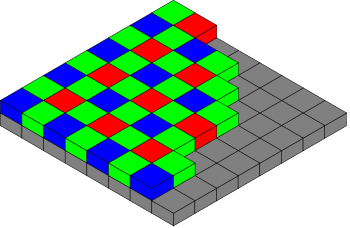
\includegraphics[width=0.35\textwidth]{figures/Bayer_pattern.png}
        \caption{Filtro de Bayer típico de un sensor CMOS-APS. Cada 4 píxeles hay 2 con filtro verde, 1 con rojo y el último con es azul.
          El color verde es utilizado dos veces debido a la sensibilidad al verde del ojo humano.}
        \label{fig:bayer}
      \end{figure}

      Si bien este filtro resulta invisible a los rayos X; %\cite{}. %TODO: La ref!
      el distinguir fotografías por sus colores permitió caracterizar
      de los distintos parámetros a la hora del tomar una fotografía,
      tal como se describe en el apéndice~\ref{sec:ap_alternatives}.

    \subsection{Detección de partículas con el sensor CMOS}\label{sec:intro:detection
    }   

      Una partícula de energía que deposite una energía $E$
      es capaz de generar $E / a$ pares de electrón-hueco en el sensor
      siendo $a$ la energía promedio para generar un par electrón-hueco en el material.
      El valor máximo de electrones hasta llegar a saturación es conocido como \emph{Full Well Capacity}.
      
      En el caso particular de los rayos X, estos interactúan con el Si principalmente por efecto fotoeléctrico,
      por lo que el fotón de energía $E$ es absorbido, y un electrón es expulsado con una energía $E-E_b$,
      siendo $E_b$ la energía de enlace del electrón ejectado (1.78 KeV para el Si)\cite{PerezCMOS}.

      Si la densidad de eventos en una imagen es baja\footnote{En relación con el tamaño de los eventos},
      es posible identificar eventos a partir de los pixeles de una vecindad,
      debido a que se desprecia la probabilidad de encontrar un píxel que haya acumulado carga de dos eventos distintos.
      En caso de haber una densidad de eventos mayor, pueden utilizarse otros métodos, como técnicas basadas en \emph{deep learning}
      e inteligencia artificial. \cite{ROE2005577} 
      
    \subsection{Fluorescencia de rayos X}\label{sec:intro:peaks}

      La emisión de rayos X característicos corresponde a la ionización de un átomo en la que un
      electrón de las primeras capas es excitado a un estado no ligado.
      En este caso un electrón de una capa superior ocupa la vacante dejada por el electrón.
      Durante este proceso, dado que la energía se conserva, se emite un fotón
      cuya energía es igual a la diferencia entre los niveles de la transisición.

      Los picos $K_\alpha$ y $K_\beta$ corresponden a las transiciones de un electrón de un estado
      $\ket{2p}$ al estado $\ket{1s}$ y a la transición $\ket{3p}$ a $\ket{1s}$, respectivamente.
      
      En el caso particular del Cu, Fe y Ca, los valores de energía de los fotones emitidos se encuentran
      en la Tabla~\ref{tab:xraypeaks}.

      \begin{table}[h]
        \centering
        \begin{tabular}{|rl|ll|l|} \hline
        \textbf{Z}  & \textbf{\small{Elem.}} & $K_{\alpha_1}$ & $K_{\alpha_2}$ & $K_\beta$ \\ \hline
        \textbf{20} & \textbf{Ca}       & 3692         & 3688         & 4012        \\
        \textbf{26} & \textbf{Fe}       & 6404         & 6391         & 7058        \\
        \textbf{29} & \textbf{Cu}       & 8048         & 8028         & 8905       \\ \hline
        \end{tabular}
        \caption{Valores de energía, en eV, de los fotones emitidos para los picos de emisión 
          $K_{\alpha}$ y $K_{\beta}$ del Ca, Fe y del Cu.\cite{xraybooklet}.}
        \label{tab:xraypeaks}
        \end{table}

    \subsection{Rayos cósmicos}\label{sec:intro:cosmic_ray}
      Los rayos cósmicos son partículas que llegan desde el espacio y bombardean constantemente la Tierra desde todas direcciones.
      La mayoría de estas partículas son protones o núcleos de átomos.
      Al interactuar con la atmósfera terrestre, estas partículas son capaces de producir hadrones cargados, neutrones,
      fotones (rayos $\gamma$), muones, electrones y positrones, \cite{GriederCRAE}
      cuyos efectos son medibles.
      %TODO: Poner algunos valorcitos

  %%%%%%%%%%%%%%%%%%%%%%%%%%%%%%%%%%%%%%%%%%%%%%%%%%%
  \section{Configuración experimental}\label{sec:conf_exp}

    \subsection{Sensor CMOS}\label{sec:conf_exp:CMOS}
      Se ha utilizado el sensor OmniVision OV5647 de la cámara Raspicam V1.3 cuyo precio ronda los 23 dólares.
      El sensor posee	$2592$x$1944$ píxeles, lo que le una resolución total de $5$ MP.
      El tamaño de un píxel de \SI{1.4}{\micro\meter} x \SI{1.4}{\micro\meter}.
      El capacidad de carga máxima hasta llegar a saturación es de $4300$ electrones (\emph{Full Well Capacity}).
      El sensor posee un ADC de 10 bits por píxel.
      El tamaño total por imagen raw es de unos \SI{6.4}{\mega\byte}

    \subsection{Raspberry}\label{sec:conf_exp:raspberry}
      Se utilizó una Raspberry Pi modelo B, con una memoria micro SD de \SI{16}{\giga\byte}, para la obtención de imágenes.
      Debido a la resolución de las imágenes, la profundidad de bits de la imagenes y del tamaño del sistema operativo \emph{Raspbian}, 
      la memoria disponible permitió almacenar del orden de 1000 fotografías en simultáneo.

    \subsection{Librería raspiraw}\label{sec:conf_exp:raspiraw}
      Para la adquisicón de datos se utilizó la librería {\it raspiraw}\cite{raspiraw} debido a la rapidez con la que se toman los datos.
      En el apéndice~\ref{sec:ap_alternatives} se muestran otras alternativas que son más lentas para la toma de datos,
      pero que pueden resultar más simples y sencillas de implementar.

      Los datos sin procesamiento (datos \emph{raw}) eran guardados con extensión raw.
      Los mismos consistian en $1952$ filas de 3264~bytes.
      Las últimas $8$ filas de datos no contienen información y no son utilizadas,
      ya que sólo existen debido a que $1952$ es menor múltiplo de $16$
      mayor a las $1944$ filas que posee el sensor (ver sección \ref{sec:conf_exp:CMOS}).
      De la misma forma, los último $24$~bits de cada fila no son utilizados y deben ser descartados.
      %TODO: Verificar la cuenta!

      El valor de carga acumulada por cada píxel se representa mediante un número de $10$~bits.
      En una misma columna, los píxeles son agrupados de a $4$, formando una estructura de $5$~bytes.
      En los primeros $4$~bytes se encuentran los bits más significativos de los 4 píxeles que conforman la estructura.
      El quinto byte contiene los últimos $2$~bits menos significativos de cada píxel.\cite{picamera}
      La manera en la que los bits están ordenados en un grupo se muestra en la Fig.~\ref{fig:arreglo}

      \begin{figure}[h]
        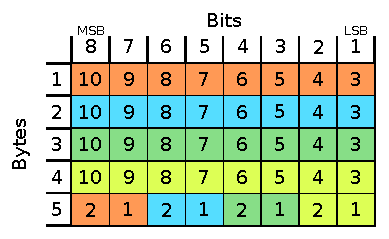
\includegraphics[width=0.47\textwidth]{figures/bayer_bytes.pdf}
        \caption[LoF entry]{Representación de un grupo 4 píxeles.

        Los $40$~bits de los $4$ píxeles están distribuídos como ilustra la figura.
        Colores distintos corresponden a píxeles distintos.

        En las filas se indica en número de byte (siendo $5$ en total).

        En cada celda se encuentra un número que representa el bit de información de un píxel,
        siendo 1 el bit menos signficativo (LSB) y 10 el bit más signficativo (MSB).}
        \label{fig:arreglo}
      \end{figure}

      Los parámetros que permite variar esta librería son:
      \paragraph{Tiempo de exposición:}
        Se define como el tiempo en el que sensor acumula carga.
        A mayor tiempo de exposición, mayor es la carga leída por el detector.
        
        En lo que sigue, se utilizó un tiempo de exposición de \SI{500}{\milli\second}, a no ser que se aclare lo contrario.

      \paragraph{Cuadros por segundos:}
        También conocido como \emph{fps} por sus siglas en inglés.
        Se refiere a la frecuencia con la que se toman las imágenes y generalmente viene expresado en fotografías por segundo.
        
        En lo que sigue, se capturó a 2 cuadros por segundo, a no ser que se aclare lo contrario.

      %\paragraph{Ganancia}

    \subsection{Emisor de rayos X}\label{sec:conf_exp:x-rays}
      En la Fig.\ref{fig:photo_xray} se muestra la configuración experimental utulizada.
      La cámara de la Raspberry Pi se colocó en un recipiente de plástico opaco a la visible
      para evitar los fotones en ese rango de longitudes de onda.
      El equipo utilizado posee dos ventanas, se utilizó la menos coherente para facilitar el proceso
      de alineado del haz con la cámara. 

      El generador de rayos X utilizado corresponde al grupo de materiales del Centro Atómico Bariloche,
      el mismo utiliza la diferencia de energía entre los niveles del Cu para generar los rayos X.
      Por este motivo, la emisión de los rayos X no corresponde a un espectro uniforme, sino que presenta
      máximos locales en los valores que corresponden a diferencias de niveles energéticos.
      
      Para la medición de los picos de Fe y Ca se intercaló una lámina de Fe y una concha marina (rica en Ca).

      \begin{figure}[h]
        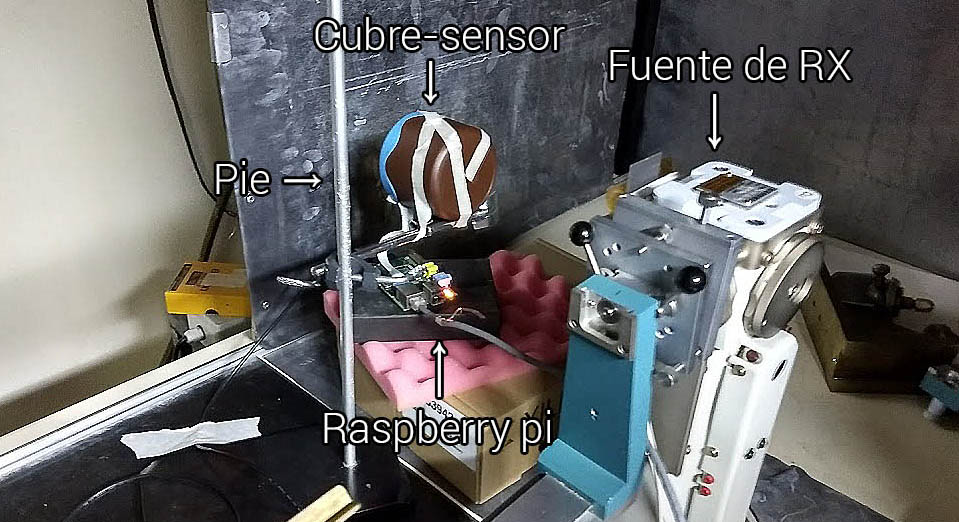
\includegraphics[width=0.47\textwidth]{figures/IMG_20180412_173110355_HDR}
        \caption{Configuración experimental utilizada. Se } %TODO: Completar
        \label{fig:photo_xray}
      \end{figure}

    \subsection{Observación de rayos cósmicos.}\label{sec:conf_exp:cosmic_ray}
      Utilizando la librería es posible idenficar eventos en paralelo con la toma de imágenes,
      por lo que se implementó un sistema que guarde solamente las imágenes que poseen pixeles que superen un umbral establecido.
      Debido al ruido de fondo, dicho umbral se ajustó en $75$ Unidades de ADC. 
      Como se verá en la sección \ref{sec:results:cosmic_ray}, con esta configuración fue posible detectar eventos,
      por lo que el umbral establecido resultó válido y suficiente.
      Se tomaron 2 imágenes por segundo, pero estas eran capaces de procesarse a una velocidad
      del orden de 1 imagen cada 3 segundos, por lo que la frecuencia de eventos debido a rayos cósmicos detectado sea menor a
      la frecuencia de eventos esperada, que es del orden de \SI{100}{\meter^{-2}\second^{-1}}.

    \subsection{Librería propia}\label{sec:conf_exp:library}
      Para el procesamiento de las imagenes de raspiraw se implementó una librería en C++. En esta librería las imágenes pasan
      a ser objetos representados por matriz (arreglo modulado). Cada foto presenta un ancho, un largo y un conjunto de datos que
      corresponder al valor de cada pixel. En esta clase se definen los métodos (funciones) para encontrar eventos, basándose en
      pixeles adyacentes, para recortar imágenes, encontrar el valor medio, la mediana y hasta para encontrar
      la desviación estándar de los valores de los pixeles.

      A su vez, cada evento es representado por otra clase cuya identidad viene dado por una lista de pixeles (posición horizontal,
      posición vertical y valor). Para esta clase se definen métodos que permiten
      obtener la carga total de un evento, definida como la suma de los valores de los pixeles;
      para obtener el centro de masa del evento,
      definida como una promedio de los vectores posiciones de cada pixel,
      ponderado con el valor del pixel;
      para determinar el radio de un evento, definido como la raiz cuadrada de la varianza de las posiciones
      de los pixeles al centro de masa, también ponderado por el valor de cada pixel.

      El código fuente puede encontrarse en la plataforma GitHub mediante el siguiente enlace
      \href{https://github.com/DBFritz/ParticleDetections}{\texttt{github.com/DBFritz/ParticleDetection}}

  %%%%%%%%%%%%%%%%%%%%%%%%%%%%%%%%%%%%%%%%%%%%%%%%%%% 
  \section{Resultados y discusión}\label{sec:results}
    Se probó el correcto funcionamiento de la librería en tres aplicaciones diferentes.
    En primer lugar se determinó el ruido de fondo de la cámara,
    otra de ellas consistió en observar los picos $K_{\alpha}$ y $K_{\beta}$ de diferentes elementos,
    y por último, en detectar Rayos Cósmicos .

    \subsection{Determinación del ruido de fondo}\label{sec:results:background}
      Se realizó un histograma de los valores de los pixeles de una única para verificar la distribución y la dispersión
      del ruido de cada imagen. Los resultados obtenidos se muestran en la Fig.~\ref{fig:histogram}

      \begin{figure}[h]
        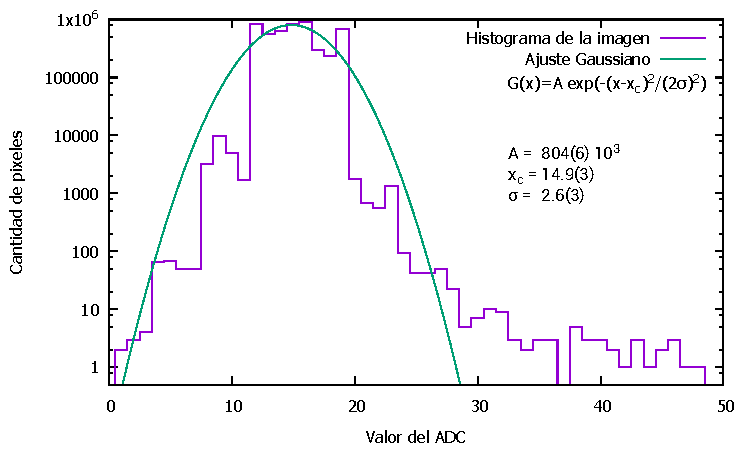
\includegraphics[width=0.45\textwidth]{figures/background_histo.pdf}
        \caption{Histograma de los valores de los pixeles con un ajuste gaussiano.
          El histograma se muestra en escala logarítmica.
          La gaussiana se encuentra centrada en $14.8(3)$ unidades de ADC,
          mientras que su dispersión es $2.5(3)$ unidades de ADC.}
        \label{fig:histogram}
      \end{figure}
      
      Se tomaron 30 imágenes con tiempo de exposición de \SI{0.5}{\milli\second} a 2 cuadros por segundos (\emph{fps}).
      Se promediaron las 30 imágenes para obtener una estimación sobre el ruido de fondo con la configuración dada. 
      En la Fig.~\ref{fig:background} se muestra el promedio por píxel de las fotografías tomadas.

      \begin{figure}[h]
        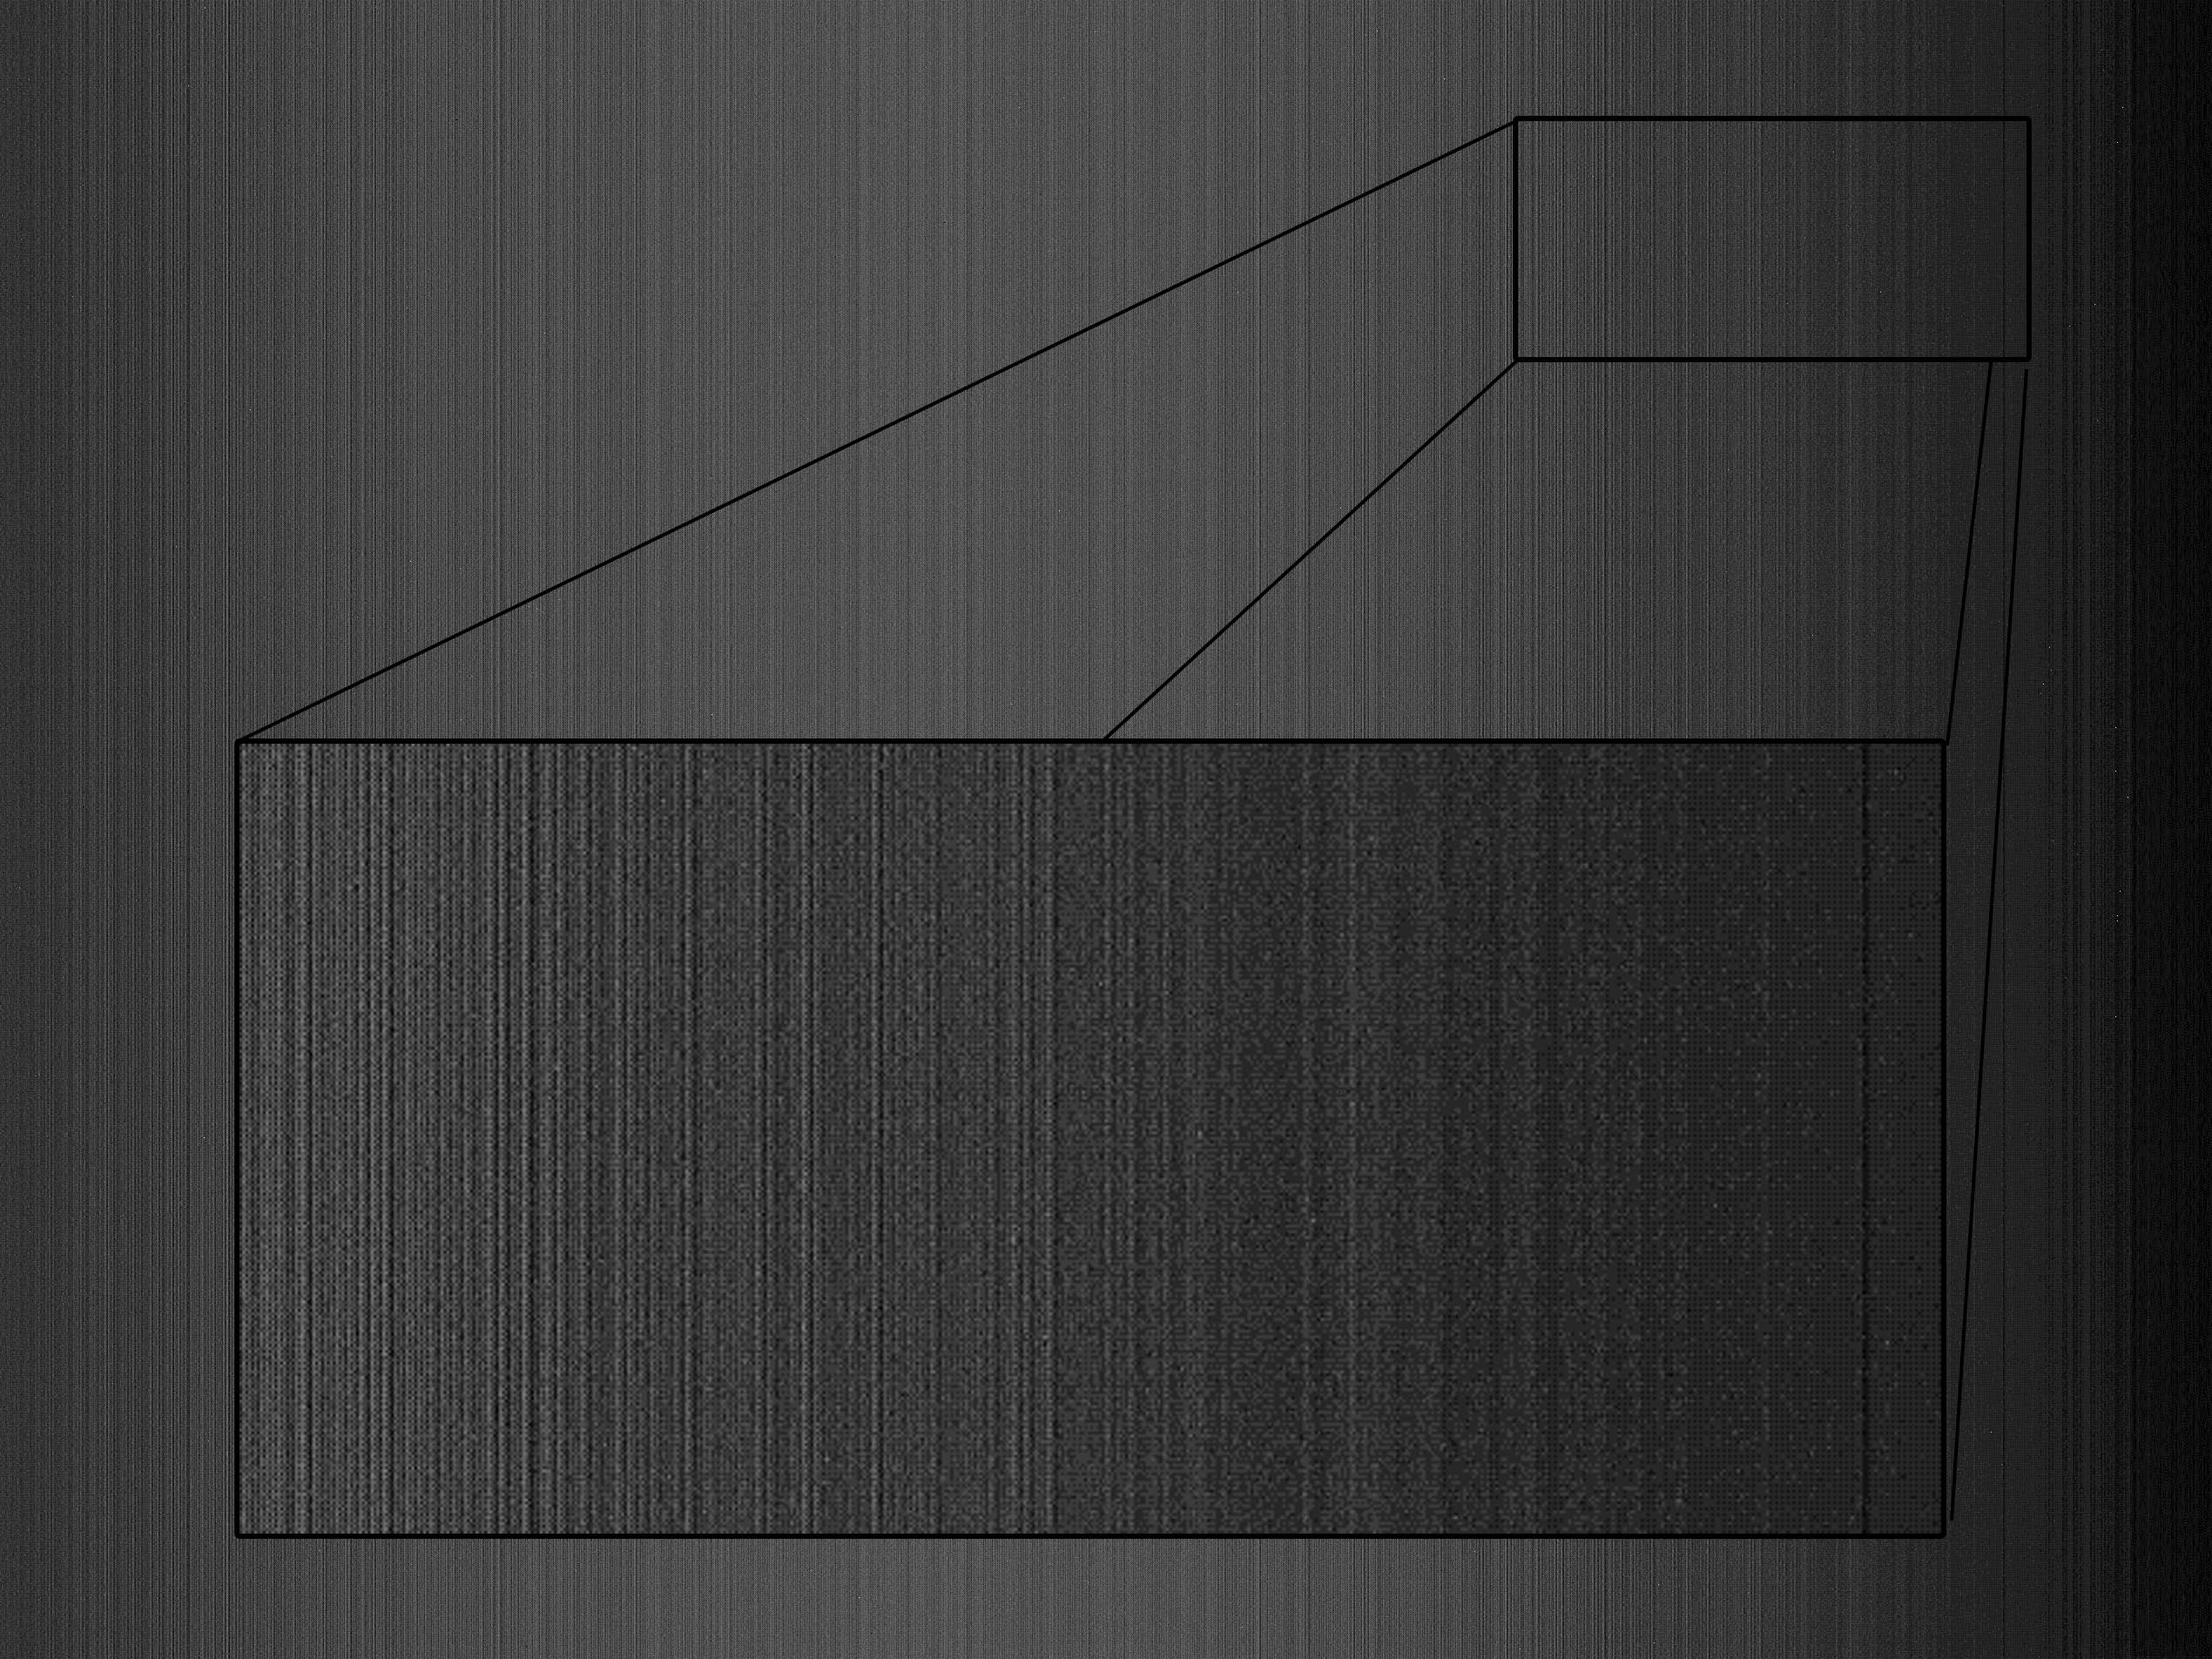
\includegraphics[width=0.47\textwidth]{figures/background.jpg}
        \caption{Promedio de las 30 imagenes.
          En la misma se observa una dependencia del valor promedio como función de la posición.
          Esta dependencia está fuertemente relacionada con la columna del píxel. }
        \label{fig:background}
      \end{figure}
      %FIXME: La foto de background.png está mal hecha, la nueva foto se encuentra en la carpeta results.
    
      En base a la fuerte dependencia del valor medio de los pixeles como función de la columna,
      se implementó una función que permite sustraer, a cada columna, la mediana por columna.
      Esto se hizo con la premisa de que, en una misma columna,
      los pixeles que poseen información de eventos son menos que el resto.
      Esta función será aplicada a cada procesamiento de datos de imágenes.
      El histograma de la misma imagen que en la Fig.~\ref{fig:histogram}, con la respectiva sustracción
      de la mediana por columna, se muestra en la Fig.~\ref{fig:histogram_subs}

      \begin{figure}[h]
        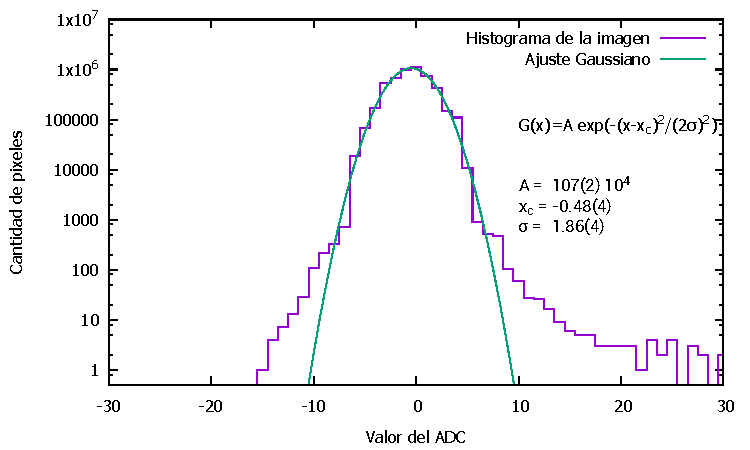
\includegraphics[width=0.47\textwidth]{figures/background_histo_subs.pdf}
        \caption{Histograma de los valores de los pixeles, con otro ajuste gaussiano.}
        \label{fig:histogram_subs} %TODO: Ampliar el caption.
      \end{figure}

    \subsection{Mediciones de picos $K_{\alpha}$ y $K_{\beta}$ y calibración de energía}\label{sec:results:peaks}
      Se analizó el espectro de Cu, Fe y Ca utilizando la librería propia.
      Para esto se realizó un histograma de la carga de los eventos.
      En estos espectros fue posible identificar los picos $K_{\alpha}$ y $K_{\beta}$ de Cu y los picos $K_{\alpha}$ del Fe y del Ca,
      esta identificación y asociación nos permitió hacer una calibración de energía como función del canal.
      tal como se muestra en la Fig.~\ref{fig:spectrum_x-ray}.
      %FIXME: Al decir esto no queda muy en claro si por qué debería atenuarse, no digo nada en la conf. experimental.
      %       Debería describir más?

      \begin{figure}[h]
        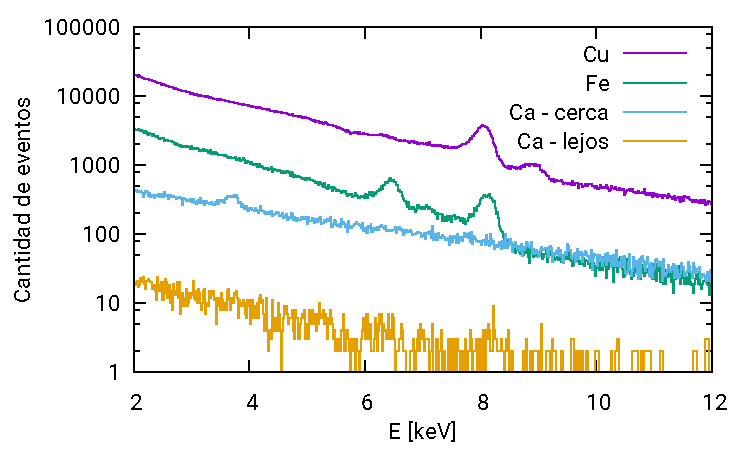
\includegraphics[width=0.47\textwidth]{figures/x-ray_spectrum.pdf}
        \caption{Espectro patronum!} %TODO: Poner caption
        \label{fig:spectrum_x-ray}
      \end{figure}

      Conociendo la energía característica de cada uno de estos picos \cite{thompson2016xray},
      y bajo la suposición que los electrones generados pierden todas su energía, % FIXME: Poner la consideración de que el fotón se frena
      se realizó una calibración del valor raw de un pixel como función de la carga (energía) depositada.
      Esta calibración se muestra en la Fig.~\ref{fig:x-ray_calibration}

      %TODO: Sacar esta porquería y explicar más cómo fue el setup experimental
      En estos gráficos no fue posible el análisis de la atenuación debido a la presencia de Fe ni de Ca
      ya que la distancia del sensor a la fuente fueron distintas en todos los casos, y por lo tanto,
      el ángulo sólido subtendido por el detector fue diferente en todos los casos.
      Un análisis más cuidadoso sobre las intensidades permitiría encontrar el coeficiente de atenuación para distintos elementos.

      \begin{figure}[h]
        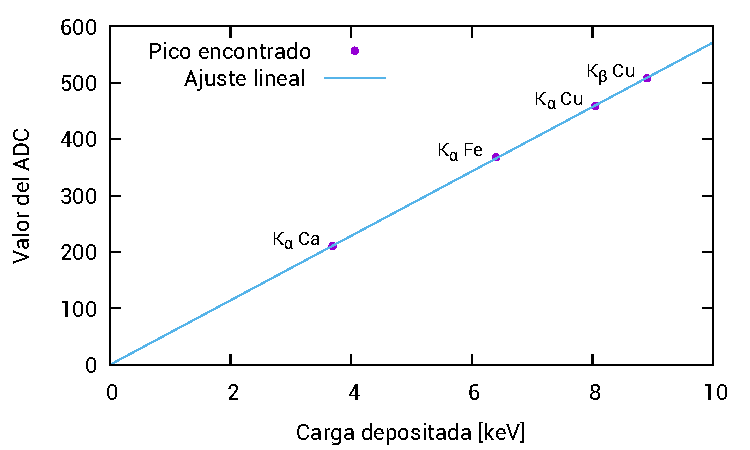
\includegraphics[width=0.47\textwidth]{figures/x-ray_calibration}
        \caption{Calibración del canal del sensor como función de la energía de
          los picos $K_{\alpha}$ y $K_{\beta}$ encontrados.
          En el mismo se puede apreciar que la relación es lineal,
          y la relación carga por unidad de ADC obtenida es de \SI{17.50(3)}{\eV} %FIXME: Poner valor
        }
        \label{fig:x-ray_calibration}
      \end{figure}

    \subsection{Medición de Rayos Cósmicos}\label{sec:results:cosmic_ray}
      Utilizando la librería se pudo encontrar $2$ %TODO: Poner el valor
      eventos en 2 días seguidos, con la cámara en oscuridad y sin la presencia de fuentes radioactivas cerca,
      por lo que se asocia estos eventos a los rayos cósmicos.
            %FIXME: No se puede asegurar que sean muones, sadly :'(
      En la Fig.~\ref{fig:cosmic_ray} se muestra uno de los eventos detectados.

      \begin{figure}[
        h]
        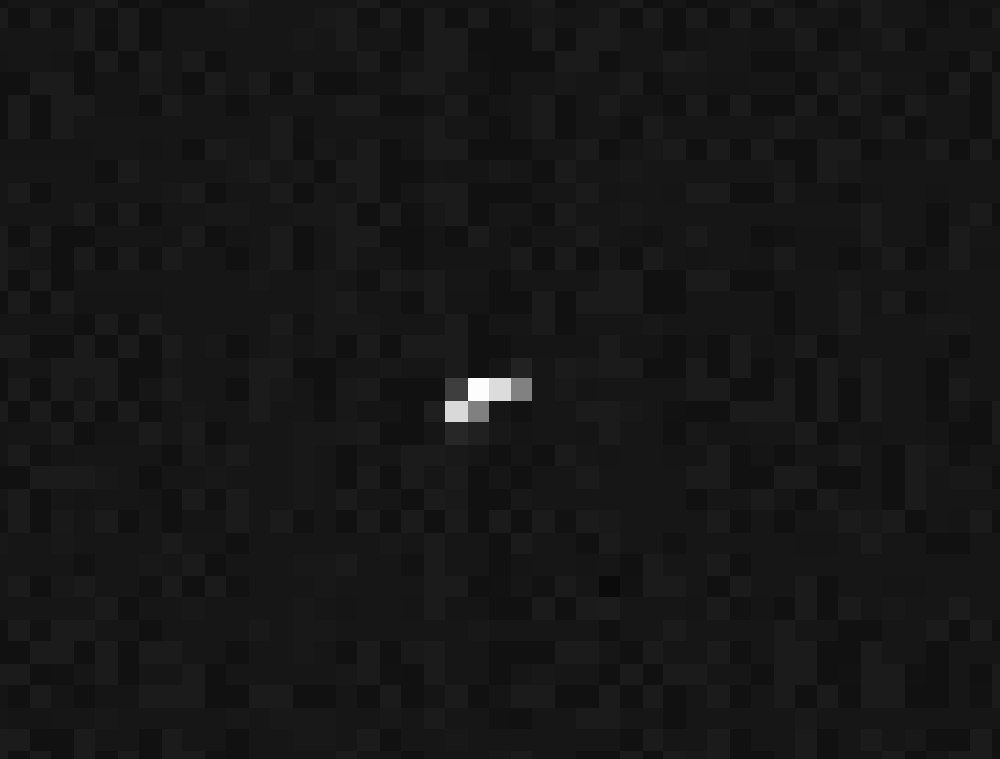
\includegraphics[width=0.47\textwidth]{figures/06-04-18_12-25-40.png} % TODO: Poner para que salga pixelada :(
        \caption{Recorte de una imagen tomada en la que se observa un evento de rayo cósmico.
        En este caso el color negro representa el 0 unidades de ADC, y el color blanco, 180 unidades de ADC.
        }
        \label{fig:cosmic_ray}
      \end{figure}

      %TODO: Hacer la cuenta!!!

  %%%%%%%%%%%%%%%%%%%%%%%%%%%%%%%%%%%%%%%%%%%%%%%%%%%
  \section{Conclusiones}
    Se utilizaron sensores CMOS para la detección de eventos con partículas para una descripción cualitativa y esquemática.
    Se analizó la dependencia con los distintos parámetros de la cámara y en base a esto se decidió una configuración de trabajo.

    Gracias a esto se pudo caracterizar y calibrar el sensor para la configuración utilizada mediante la implementación de la librería
    en C++ con filosofía de Programación Orientada a Objetos.
    Utilizando esta librería se observó la presencia de eventos producidos por rayos cósmicos y
    se observaron los picos $K_{\alpha}$ y $K_{\beta}$ del Cu y los picos $K_{\alpha}$ del Fe y Ca.

  %%%%%%%%%%%%%%%%%%%%%%%%%%%%%%%%%%%%%%%%%%%%%%%%%%% 
  \bibliographystyle{unsrt}
  \bibliography{bibliography}

  %%%%%%%%%%%%%%%%%%%%%%%%%%%%%%%%%%%%%%%%%%%%%%%%%%%
  \section*{Agradecimientos}
    Se agradece la colaboración de Xavier Bertou por la experiencia brindada y por
    acompañar el trabajo en forma constante.
    A Miguel Sofo por la disponibilidad y por la ayuda a la hora de hacer mediciones.
    % TODO: Agregar a alguien que Bertou me dijo pero me colgué
    % Era del grupo de José por proveernos de los rayos X
    Al equipo de Fabricio Alcalde por proveernos e informarnos sobre el equipo de rayos X.

  %%%%%%%%%%%%%%%%%%%%%%%%%%%%%%%%%%%%%%%%%%%%%%%%%%%
  \clearpage
  \appendix
  \section{Alternativas a Raspiraw}\label{sec:ap_alternatives}
  
  \subsection{Raspistill y Raspivid}
    Ambos vienen por defectos instalados en el sistema operativo \emph{Raspbian}.
    Raspistill permite capturar fotografías en formato \emph{Joint Photographic Experts Group} (jpeg/jpg).
    Si bien las imágenes tomadas presentan un post-procesamiento, Rapistill es capaz de añadir a la imagen los datos sin procesar (\emph{raw}),

    Por el otro lado, raspivid permite grabar videos en formato \emph{H.264}.
    Este formato también presenta compresión de datos, al igual que .jpg, pero no existe parámetro que permita obtener las imágenes sin procesamiento.
    Por lo debe ser utilizado de manera ilustrativa y cuantitativa, pero no cuantitativa.

    Para verificar el funcionamiento de la cámara se expuso la cámara ante una fuente de rayos alfa.
    Utilizando raspivid, se tomó 1 minuto de exposición a 30 cuadros por segundos.
    Por pixel, se tomó el máximo valor de las 1800 imágenes, generando la imagen que se muestra en la Fig.~\ref{fig:raspivid}

    \begin{figure}[h]
      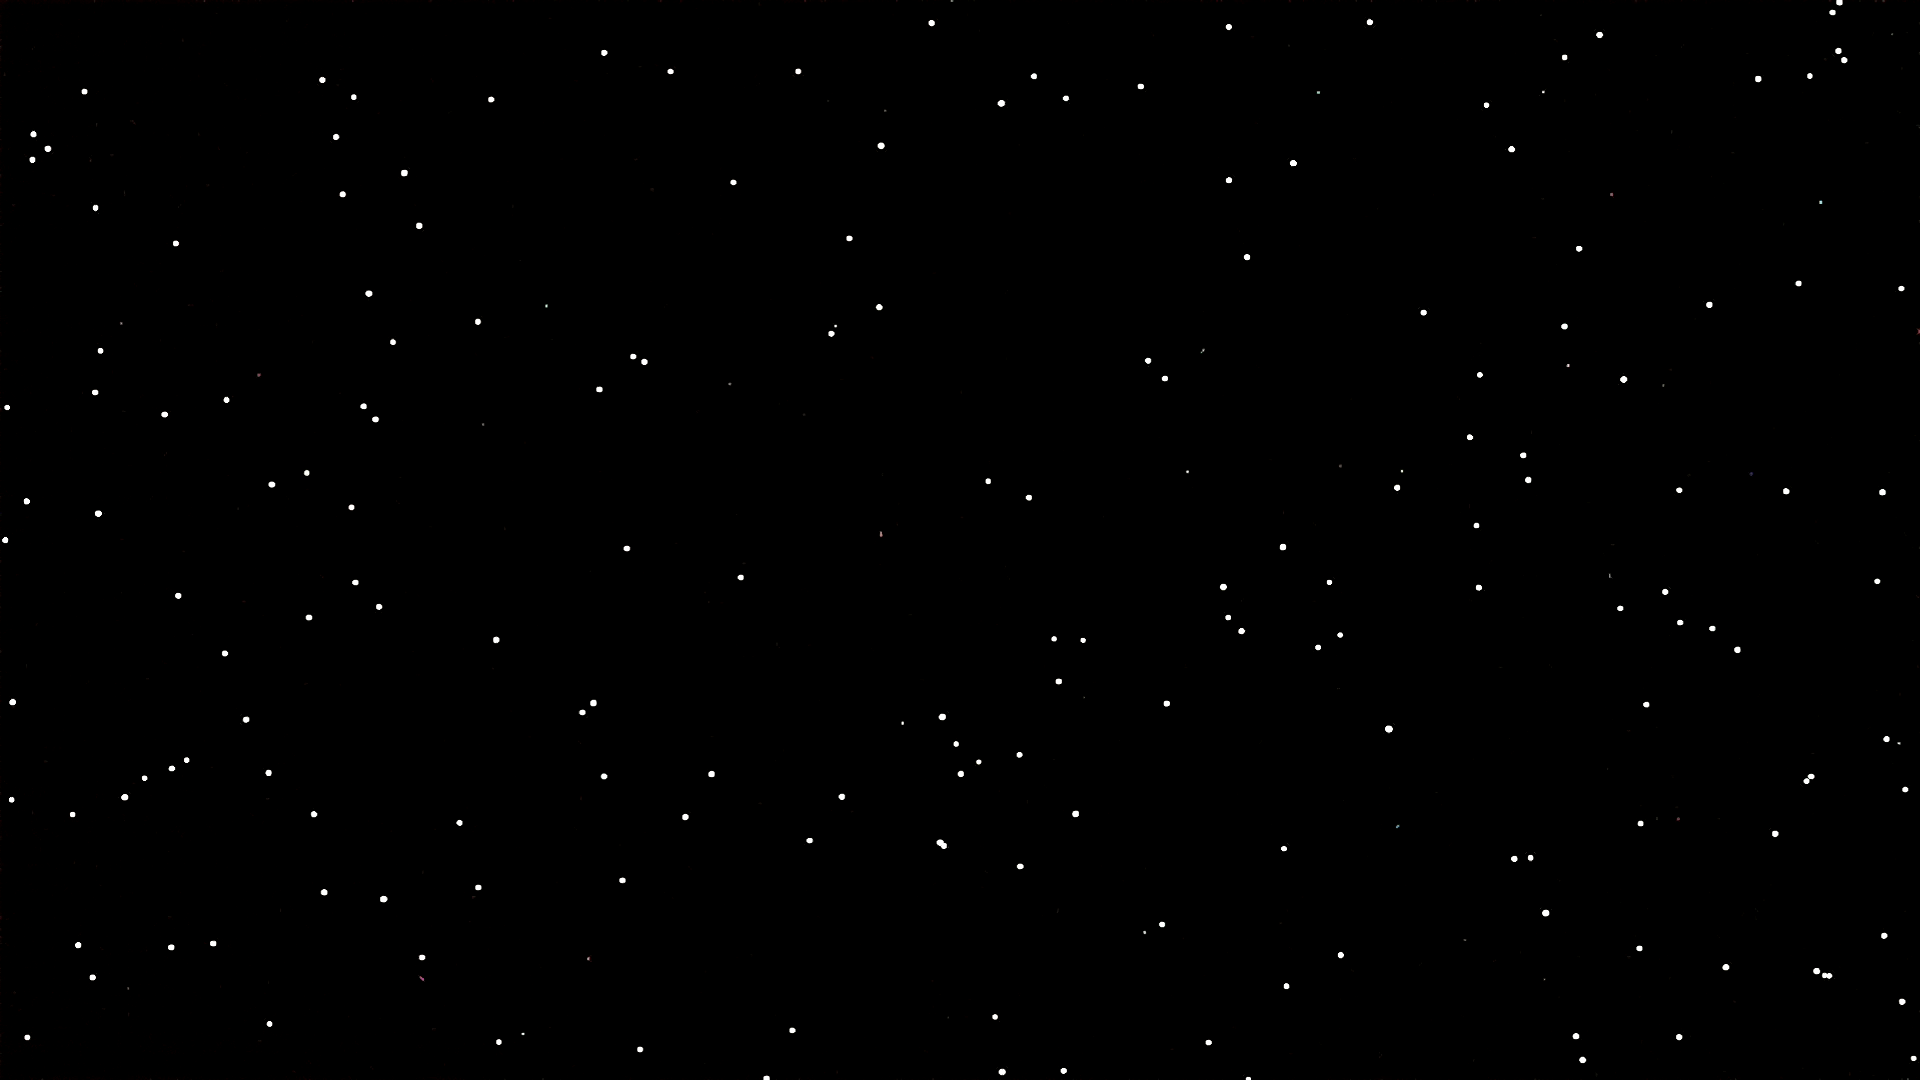
\includegraphics[width=0.47\textwidth]{figures/Alpha_1m.png} % TODO: Poner para que salga pixelada :(
      \caption{Imagen de los eventos con exposición de 1 minuto ante una fuente de $^{241}$Am,
      que emite radiación alfa de \SI{5.486}{\mega\eV}.
      Para la composición de la misma se tomó el valor máximo por pixel de cada fotograma del video.
      } %TODO: Pongo la equivalencia en electrones?
      \label{fig:raspivid}
    \end{figure}

  \subsection{Picamera, librería en Python} % TODO: Terminar esta porquería
    La librería Picamera presenta en su documentación una forma para obtener los datos \emph{raw}, sin procesamiento previo.
    Esta librería, debido a que está dedicada para la toma de fotografías, permite controlar los valores de ISO, tiempo de exposición,
    balance de blancos.

    Como primera aproximación al estudio de los datos \emph{raw}, se analizó la dependencia de los histogramas de los valores de los píxeles.
    En primer lugar se estudio la dependencia con el ISO, tal como se muestra en la Fig.~\ref{fig:ISO}

    Luego se analizó la dependencia del histograma para distintos valores de balance de blancos.
    Se observó que los valores de los datos \emph{raw}, no depende del balance de blancos;
    lo que indica que el balance de blancos es un post-procesamiento.
    Tal como se muestra en la Fig.~\ref{fig:WB}

    \begin{figure}[h]
      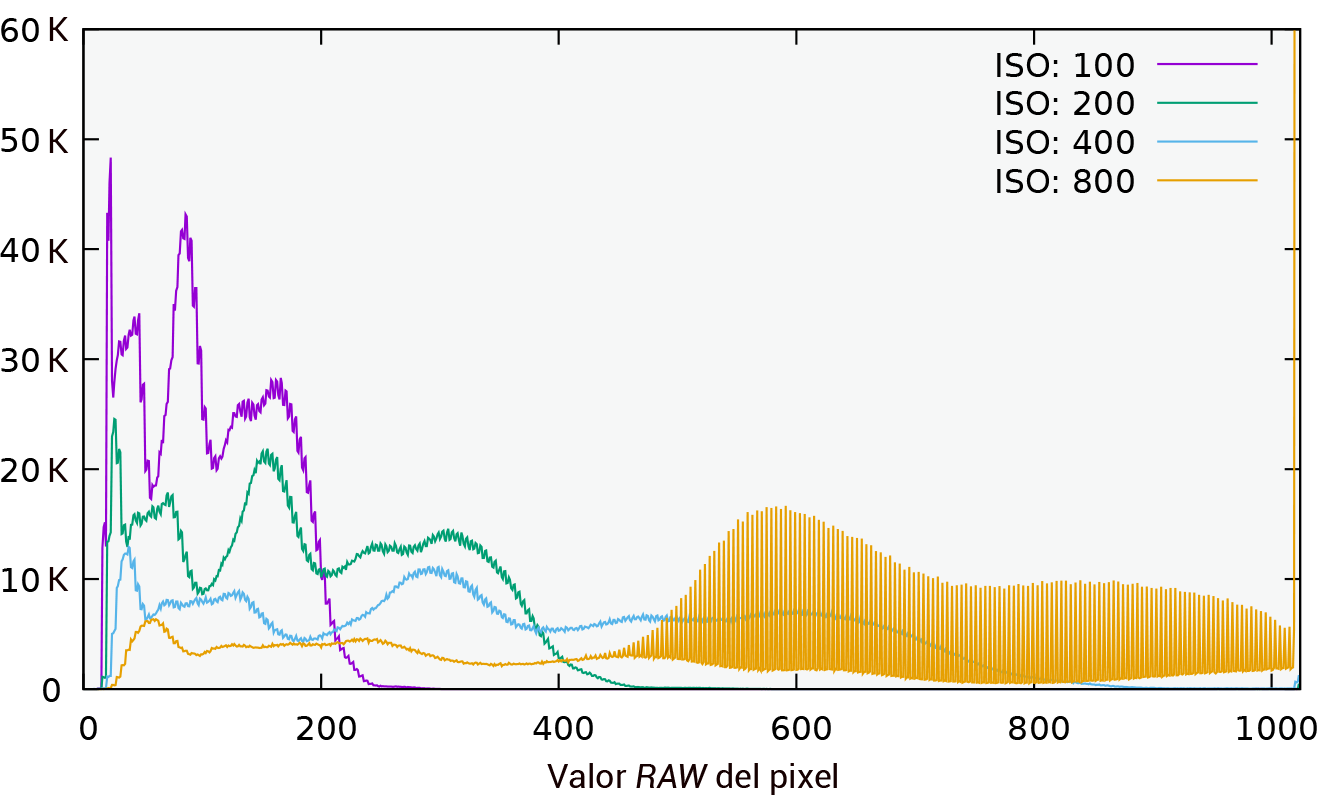
\includegraphics[width=0.47\textwidth]{figures/ISO.png}
      \caption{Vale por un caption.
      }
      \label{fig:ISO}
    \end{figure}

    \begin{figure}[h]
      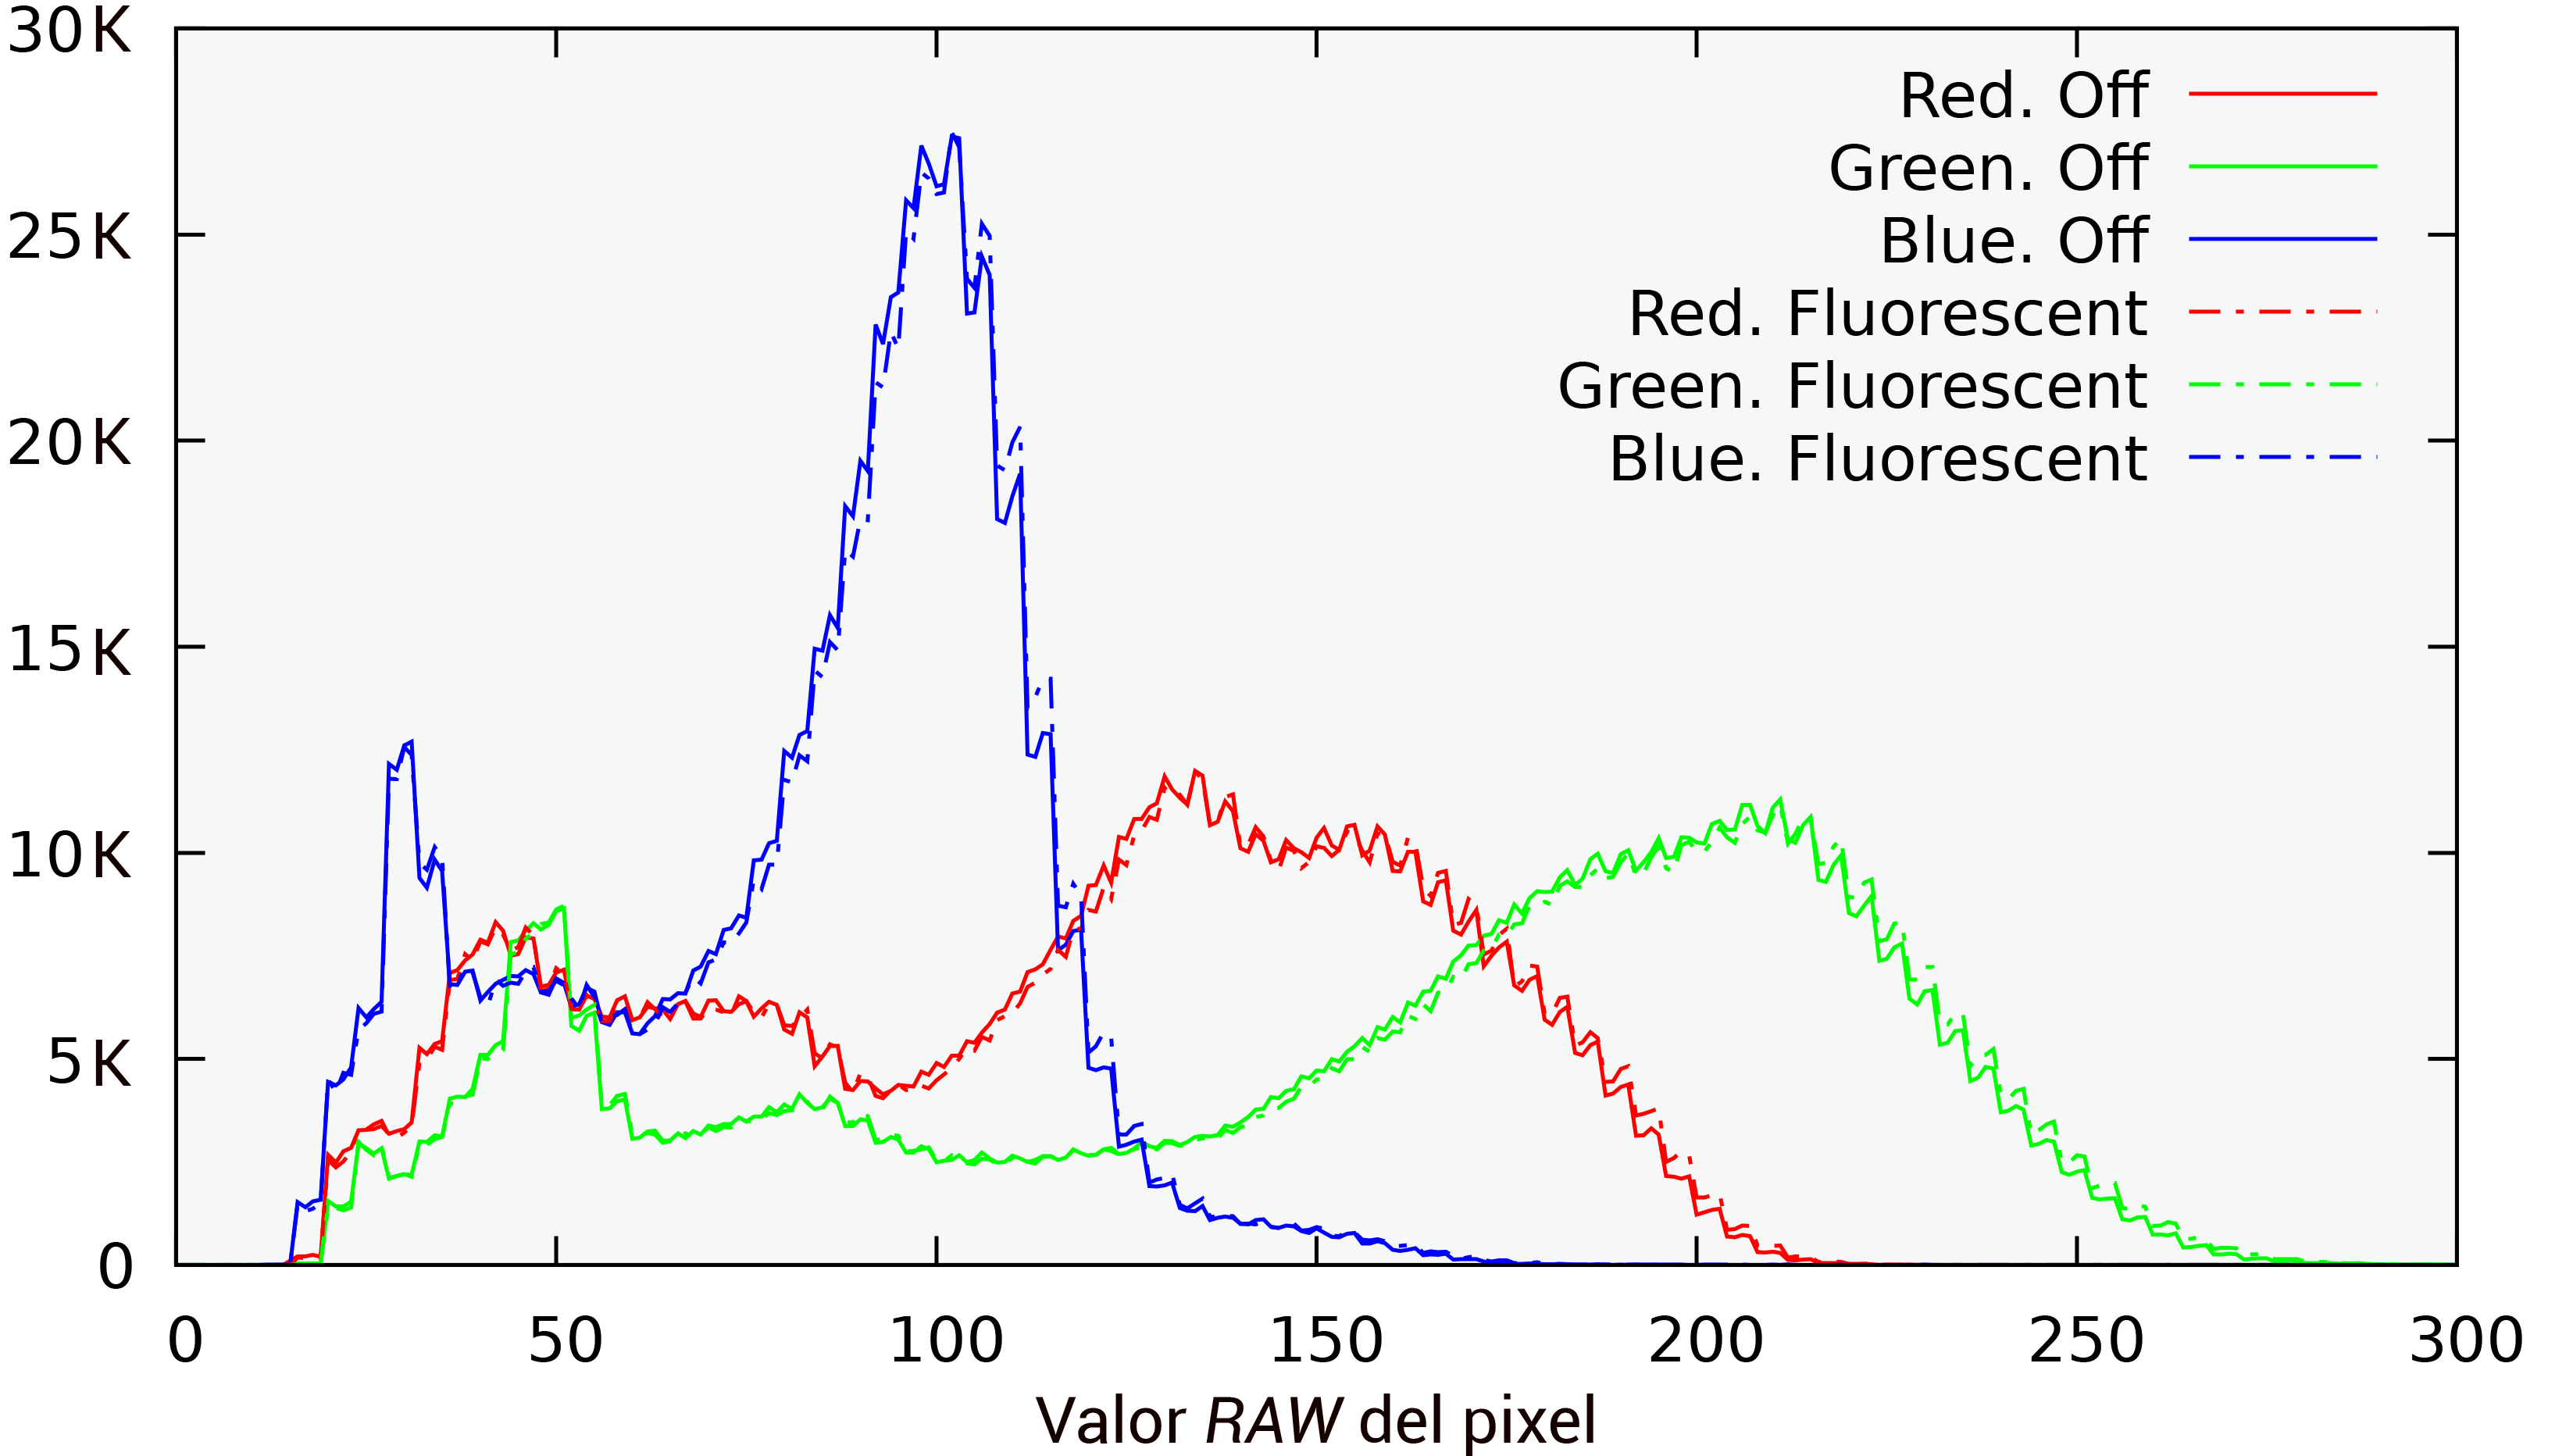
\includegraphics[width=0.47\textwidth]{figures/WB_component_transparent.png}
      \caption{Vale por un caption.
      }
      \label{fig:WB}
    \end{figure}

    %TODO: Completar

\end{document}

    



